\section{Dissimilarity Constraint} \label{sec:dissimilarityconstraint}

\input{fig/dissimilarity_statistic.tex}

To compute this statistic, we randomly sampled 5000 target tags.
Then, for each target tag we randomly sampled tags until we found a secondarily-sampled tag that was within a 0.01 match distance radius of the target and a secondarily-sampled tag that was outside a 0.99 match distance radius of the target.
Finally, we computed the match distance between the pair of secondarily-sampled tags.
Figure \ref{fig:dissimilarity_statistic} summarizes this process.

\begin{figure}
\begin{center}

\begin{subfigure}[b]{\columnwidth}
\centering
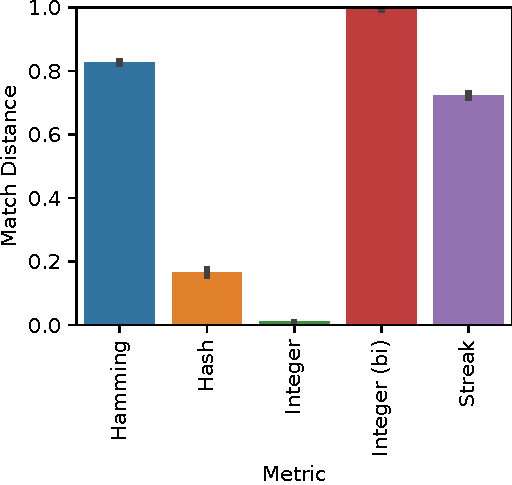
\includegraphics[width=\columnwidth]{{{sphere_reverse/bitweight=0.5+seed=1+title=dimensionality_barplot+_data_hathash_hash=7eaa832497d2f3cb+_script_fullcat_hash=03ce1e318a24a109+ext=}}}
\caption{
TODO
}
\label{fig:sphere_reverse_distnplot}
\end{subfigure}


\begin{subfigure}[b]{\columnwidth}
\centering
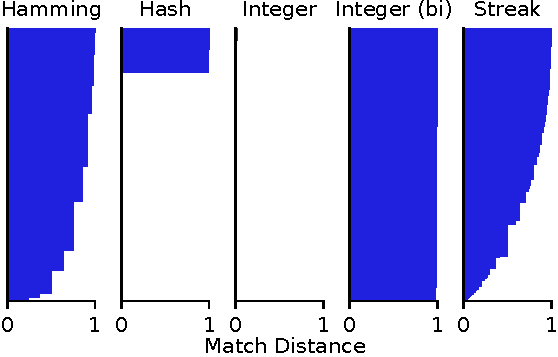
\includegraphics[width=\columnwidth]{{{sphere_reverse/bitweight=0.5+seed=1+title=dimensionality_distnplot+_data_hathash_hash=7eaa832497d2f3cb+_script_fullcat_hash=03ce1e318a24a109+ext=}}}
\caption{
TODO
}
\label{fig:sphere_reverse_barplot}
\end{subfigure}

\caption{
TODO
}
\label{fig:sphere_reverse}

\end{center}
\end{figure}


Supplementary Figure \ref{fig:sphere_barplot} provides our estimate of the dissimilarity constraint statistic for each metric, with error bars representing a 95\% confidence interval.
Supplementary Figure \ref{fig:sphere_distnplot} shows the distribution of the dissimilarity constraint statistic values among the 5000 replicate samples in greater detail.

These results tell a story across metrics very to the simiarity constraint results.
The hash metric exhibited no geometric structure.
The streak metric exhibited some geometric structure in the mean case (mean secondarily-sampled distance 0.7127), but outcomes that strongly broke geometric constraints were also observed (we observed distances between secondarily-sampled tags as low as 0.0002).
The hamming metric exhibited stronger geometric structure in the mean case (mean secondarily-sampled distance 0.8248) and had less extreme tail-end outcomes (we observed match distances between the secondarily-sampled tags only as low as 0.2355).
The bidirectional integer metric was highly constrained in both the mean and tail-end cases.
The smallest distance between secondarily-sampled tags was 0.9802.
Again, the unidirectional integer metric exhibited a quirky result due to its noncommutative nature.
The mean distance between secondarily-sampled tags was 0.0100.
As shown in Figure \ref{fig:sphere_distnplot}, all secondarily-sampled distances oberved with this metric were extremely small.
Under this metric, if you sample a tag that is close to a target it will be numerically slightly larger than the target.
Likewise, if you sample a tag that is very far from a target, it will be numerically slightly smaller than the target (due to wraparound).
Then, explaining this counterintuitive result, the distance from the slightly smaller to the larger tag will be small.
